\section{List Diagnosis under Training Interventions}
\label{sec:diagnosis}

% D1: Confirmation contrast; strict counts and target positions.
Figure~\ref{fig:preference-position} compares the three training/fusion conditions on the same 371 covered confirmation queries. E0 obtains 208 strict preferences (56.06\%), compared with fusion's 189 (50.94\%), yet its preferred-passage MRR is 0.3169 versus 0.6017. The mean ranks of the preferred passage and its counterpart are 81.91/96.27 for E0 and 3.45/3.70 for fusion. Both designated passages occur in the top 10 for only 12 queries under E0, compared with 348 under fusion. Thus, E0's higher preference count coexists with substantially deeper designated-passage positions; it is not evidence of better ordering of the full pool.

\begin{figure}[b]
\centering
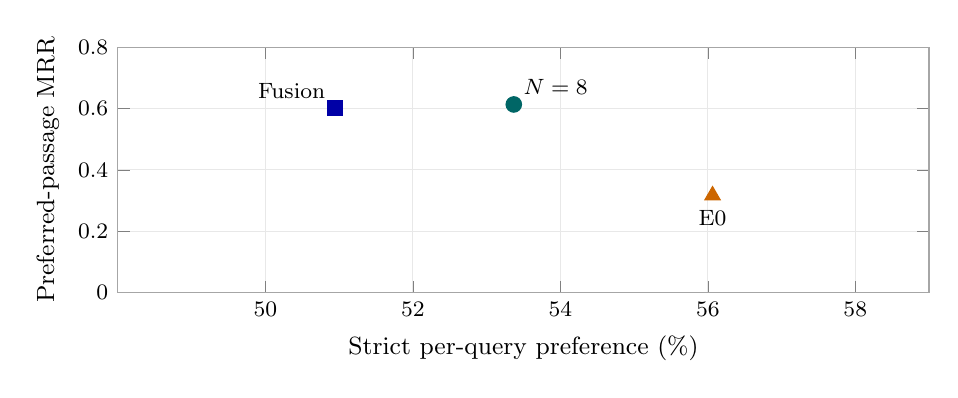
\begin{tikzpicture}
\begin{axis}[
width=0.98\columnwidth,height=4.7cm,
xmin=48,xmax=59,ymin=0,ymax=0.8,
xtick={50,52,54,56,58},ytick={0,0.2,0.4,0.6,0.8},
xlabel={Strict per-query preference (\%)},
ylabel={Preferred-passage MRR},
label style={font=\small},tick label style={font=\footnotesize},
grid=major,grid style={gray!18},axis line style={gray!70},
enlargelimits=false,clip=false]
\addplot[only marks,mark=square*,mark size=2.8pt,color=blue!65!black]
coordinates {(50.9433962264,0.601666468764)};
\node[anchor=south east,font=\footnotesize] at (axis cs:50.9433962264,0.601666468764) {Fusion};
\addplot[only marks,mark=triangle*,mark size=3.2pt,color=orange!80!black]
coordinates {(56.0646900270,0.316875873524)};
\node[anchor=north,font=\footnotesize] at (axis cs:56.0646900270,0.300875873524) {E0};
\addplot[only marks,mark=*,mark size=2.8pt,color=teal!80!black]
coordinates {(53.3692722372,0.613318815307)};
\node[anchor=south west,font=\footnotesize] at (axis cs:53.3692722372,0.613318815307) {$N=8$};
\end{axis}
\end{tikzpicture}
\caption{Preference and preferred-passage position on the same confirmation population ($n=371$). Higher is better on both axes. Points are observed aggregates; they do not show uncertainty intervals or establish causal mechanisms.}
\label{fig:preference-position}
\end{figure}

% D2: Joint background intervention and preserved negative result.
Background training recovers designated-passage positions while losing some of E0's strict preferences. With $N=8$, preferred MRR reaches 0.6133, mean ranks are 2.49/2.82, and both passages appear in the top 10 for 363 queries. Strict correctness falls to 198/371, ten below E0. Relative to fusion, this variant has nine more correct preferences, but its preferred-at-1 count is one lower (135 versus 136). Development exhibits the same directional tradeoff against E0: MRR increases from 0.2851 to 0.5731 while strict correctness decreases from 44/74 to 39/74. Development was used for stopping, so this is not a second holdout validation.

% D3: Reproduction scope and unisolated mechanism.
The confirmation and development aggregates were reproduced locally from the saved models and candidate inputs; E0's pool scores exactly matched the earlier cache. The results are consistent with the revised supervision encouraging designated passages to outrank sampled background. They do not establish that all sampled candidates are irrelevant or identify which component of the joint intervention drives recovery. Only one background count and seed were evaluated, and no result here establishes the necessity of this intervention or its superiority over bounded text reranking.

% D4: What this evidence answers and what remains open.
These comparisons answer RQ1 at the level of the observed setting: the methods' ordering by strict preference differs from their ordering by designated-passage position. Both outcomes should therefore accompany the RQ2 comparison, together with separately measured costs. Planned error-category judgments and controlled rewrites can test more specific semantic hypotheses; no such explanation is inferred from these aggregate shifts alone.
